% statistics_and_probability:x13 GDC:YES
\begin{question}
  \hspace*{\fill} [Note maximale: 17]\par
  \noindent La masse M de pommes, en grammes, est normalement distribuée avec une moyenne $\mu$. Le tableau suivant montre les probabilités pour des valeurs de M.\par
  \medskip
  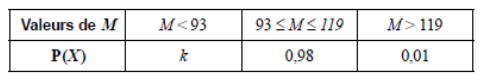
\includegraphics[scale=0.5]{tableau_de_pommes}\par
  \medskip
  (a)\par
  \medskip
  \hspace{1em}(i)  Écrivez la valeur de k.\par
  \medskip
  \hspace{1em}(ii) Montrez que $\mu = 106$.\hspace*{\fill} [4]\par
  \medskip
  (b) Trouvez $ P(M < 95)$\hspace*{\fill} [5]\par
  \medskip
  \noindent Les pommes sont emballées dans des sacs de dix.\par
  \noindent Toute pomme dont la masse est inférieure à 95 g est classée comme étant petite.\par
  \medskip
  (c) Trouvez la probabilité qu’un sac de pommes choisi au hasard contienne au plus une petite pomme.\hspace*{\fill} [3]\par
  \medskip
  (d) Une caisse contient 50 sacs de pommes. Une caisse est choisie au hasard.\par
  \medskip
  \hspace{1em}(i)  Trouvez le nombre espéré de sacs de cette caisse qui contiennent au plus une petite
pomme.\par  
  \medskip
  \hspace{1em}(ii) Trouvez la probabilité qu’au moins 48 sacs de cette caisse contiennent au plus une petite
pomme.\hspace*{\fill} [5]\par
  \bigskip

\end{question}

